\documentclass[12pt,a4paper]{article}

% ─── Page Layout ───────────────────────────────────────────────────────────────
\usepackage[a4paper, margin=0.8in, headheight=14pt]{geometry}

% ─── Fonts (XeLaTeX) ───────────────────────────────────────────────────────────
\usepackage{fontspec}
\usepackage{unicode-math}
\setmainfont{TeX Gyre Pagella}
\setmonofont[Scale=0.88]{TeX Gyre Cursor}
\setmathfont{Latin Modern Math}

% ─── Packages ──────────────────────────────────────────────────────────────────
\usepackage{xcolor}
\usepackage{colortbl}
\usepackage{titlesec}
\usepackage{enumitem}
\usepackage{tabularx}
\usepackage{booktabs}
\usepackage{array}
\usepackage{amsmath}
\usepackage{tikz}
\usetikzlibrary{shapes.geometric, arrows.meta, positioning, calc, fit, decorations.pathreplacing, decorations.pathmorphing}
\usepackage{tcolorbox}
\tcbuselibrary{skins, breakable}
\usepackage{hyperref}
\usepackage{fancyhdr}
\usepackage{graphicx}
\usepackage{microtype}
\hyphenpenalty=10000
\exhyphenpenalty=10000
\sloppy
\usepackage{caption}
\usepackage{setspace}
\usepackage{multirow}
\usepackage{tocloft}

% ─── Q&A helper ────────────────────────────────────────────────────────────────
\newcommand{\Q}[1]{\textbf{#1}\par\noindent\ignorespaces}

% ─── Colour Palette ────────────────────────────────────────────────────────────
\definecolor{myred}{RGB}{196,30,58}
\definecolor{mydark}{RGB}{30,30,50}
\definecolor{mygreen}{RGB}{14,120,80}
\definecolor{myteal}{RGB}{0,130,140}
\definecolor{myamber}{RGB}{180,100,0}
\definecolor{mypurple}{RGB}{100,30,160}
\definecolor{mygray}{RGB}{246,247,249}
\definecolor{mgframe}{RGB}{180,185,200}
\definecolor{watermark}{RGB}{145,150,170}
\definecolor{hdrred}{RGB}{250,232,235}
\definecolor{hdrgreen}{RGB}{220,244,233}
\definecolor{hdrteal}{RGB}{220,242,244}
\definecolor{hdramber}{RGB}{253,242,215}
\definecolor{hdrpurple}{RGB}{238,228,255}
\definecolor{hdrgray}{RGB}{238,240,245}
\definecolor{rowalt}{RGB}{250,251,253}

% ─── Section Formatting ────────────────────────────────────────────────────────
\titleformat{\section}
  {\large\bfseries\color{myred}}{\thesection.}{0.5em}{}
  [\vspace{1pt}{\color{myred}\rule{\linewidth}{0.8pt}}]
\titleformat{\subsection}
  {\normalsize\bfseries\color{myteal}}{\thesubsection}{0.5em}{}
\titlespacing*{\section}{0pt}{18pt}{7pt}
\titlespacing*{\subsection}{0pt}{11pt}{4pt}

% ─── Paragraph ─────────────────────────────────────────────────────────────────
\setlength{\parindent}{0pt}
\setlength{\parskip}{4pt}

% ─── TOC Styling ───────────────────────────────────────────────────────────────
\renewcommand{\cfttoctitlefont}{\large\bfseries\color{myred}}
\renewcommand{\cftaftertoctitle}{\par\noindent{\color{myred}\rule{\linewidth}{0.8pt}}}
\setlength{\cftbeforetoctitleskip}{0pt}
\setlength{\cftaftertoctitleskip}{6pt}
\renewcommand{\cftsecfont}{\normalsize\bfseries\color{mydark}}
\renewcommand{\cftsecpagefont}{\normalsize\bfseries\color{mydark}}
\renewcommand{\cftsecleader}{\cftdotfill{\cftdotsep}}
\setlength{\cftbeforesecskip}{7pt}
\renewcommand{\cftsubsecfont}{\small\color{mydark}}
\renewcommand{\cftsubsecpagefont}{\small\color{mydark}}
\setlength{\cftbeforesubsecskip}{3pt}
\setlength{\cftsubsecindent}{1.4em}

% ─── Table helpers ─────────────────────────────────────────────────────────────
\renewcommand{\arraystretch}{1.45}
\setlength{\tabcolsep}{6pt}
\arrayrulecolor{mydark}
\newcolumntype{B}[1]{>{\small\bfseries\raggedright\arraybackslash}m{#1}}
\newcolumntype{C}[1]{>{\centering\arraybackslash}m{#1}}
\newcolumntype{Y}{>{\small\raggedright\arraybackslash}X}
\renewcommand{\tabularxcolumn}[1]{m{#1}}

% ─── Header / Footer ───────────────────────────────────────────────────────────
\pagestyle{fancy}
\fancyhf{}
\fancyhead[L]{\small\color{myred}\textbf{OE-EC704A}\;\color{mydark}--- Web Technology}
\fancyhead[R]{\small\color{myteal}\textbf{Module 3 Notes}}
\fancyfoot[C]{\small\color{mydark}\thepage}
\fancyfoot[R]{\small\color{watermark}\textit{\copyright\ Biraj}}
\renewcommand{\headrulewidth}{0.5pt}
\renewcommand{\footrulewidth}{0.3pt}

% ─── Hyperref ──────────────────────────────────────────────────────────────────
\hypersetup{
  colorlinks=true, linkcolor=myteal, urlcolor=myteal,
  pdfauthor={Biraj Sarkar},
  pdftitle={OE-EC704A --- Module 3 Notes}
}

% ─── tcolorbox styles ──────────────────────────────────────────────────────────
\tcbset{
  tikzbox/.style={
    colback=mygray, colframe=mgframe, boxrule=0.6pt, arc=4pt,
    left=8pt, right=8pt, top=6pt, bottom=6pt,
    colbacktitle=mgframe, coltitle=mydark,
    fonttitle=\small\bfseries
  },
  defbox/.style={
    colback=hdrgreen, colframe=mygreen, boxrule=0.8pt, arc=4pt,
    left=9pt, right=9pt, top=6pt, bottom=6pt,
    colbacktitle=mygreen, coltitle=white,
    fonttitle=\small\bfseries
  },
  formulabox/.style={
    colback=hdrteal, colframe=myteal, boxrule=0.8pt, arc=4pt,
    left=9pt, right=9pt, top=7pt, bottom=7pt,
    colbacktitle=myteal, coltitle=white,
    fonttitle=\small\bfseries
  },
  examplebox/.style={
    colback=hdramber, colframe=myamber, boxrule=0.8pt, arc=4pt,
    left=9pt, right=9pt, top=6pt, bottom=6pt,
    colbacktitle=myamber, coltitle=white,
    fonttitle=\small\bfseries
  },
  masonbox/.style={
    colback=hdrpurple, colframe=mypurple, boxrule=0.8pt, arc=4pt,
    left=9pt, right=9pt, top=6pt, bottom=6pt,
    colbacktitle=mypurple, coltitle=white,
    fonttitle=\small\bfseries
  },
  exambox/.style={
    colback=hdrpurple, colframe=mypurple, boxrule=1pt, arc=5pt,
    left=10pt, right=10pt, top=8pt, bottom=8pt,
    colbacktitle=mypurple, coltitle=white,
    fonttitle=\bfseries,
    breakable, title after break={\textbf{Frequently Asked / Viva Questions (contd.)}}}
}
\tcbset{breakable}

% ─── TikZ styles ───────────────────────────────────────────────────────────────
\tikzset{
  block/.style={rectangle, draw=myteal, fill=hdrteal,
    text width=2.5cm, align=center, minimum height=1.0cm,
    font=\small, rounded corners=3pt, line width=0.7pt},
  redblock/.style={rectangle, draw=myred, fill=hdrred,
    text width=2.5cm, align=center, minimum height=1.0cm,
    font=\small, rounded corners=3pt, line width=0.7pt},
  netnode/.style={rectangle, draw=myteal, fill=hdrteal,
    text width=1.8cm, align=center, minimum height=0.8cm,
    font=\small, rounded corners=3pt, line width=0.7pt},
  sumjunc/.style={circle, draw=myamber, fill=hdramber,
    minimum size=0.6cm, font=\small, line width=0.8pt},
  snode/.style={circle, draw=mypurple, fill=hdrpurple,
    minimum size=0.55cm, font=\footnotesize, line width=0.7pt},
  arrow/.style={-Stealth, thick, color=mydark},
  redarrow/.style={-Stealth, thick, color=myred},
  line/.style={thick, color=mydark}
}

% ═══════════════════════════════════════════════════════════════════════════════
\begin{document}
% ═══════════════════════════════════════════════════════════════════════════════

\begin{center}
  {\LARGE\bfseries\color{myred} OE-EC704A --- Web Technology}\\[5pt]
  {\normalsize\color{mydark} Semester VII \quad$\bullet$\quad 3L:0T:0P \quad$\bullet$\quad 3 Credits}\\[3pt]
  {\normalsize\color{myteal}\textbf{Module 3 Exam Notes: OOP Principles, Inheritance, Polymorphism, Packages \& Interfaces}}\\[3pt]
  {\small\color{mydark} CGEC \;$|$\; B.Tech ECE (2023--27) \;$|$\; \textit{Biraj Sarkar}}
\end{center}
\vspace{2pt}
\noindent{\color{myred}\rule{\linewidth}{1.5pt}}
\vspace{2pt}

\hypersetup{linkcolor=mydark}
\tableofcontents
\hypersetup{linkcolor=myteal}
\newpage

% ===============================================================================
\section{Core Object-Oriented Programming (OOP) Principles}
% ===============================================================================

Java is a pure object-oriented programming language designed around four fundamental concepts.

\begin{tcolorbox}[defbox, title={\textbf{The Four Pillars of Object-Oriented Programming}}]
\begin{enumerate}[leftmargin=*, itemsep=4pt]
  \item \textbf{Encapsulation (Data Hiding):} Wrapping variables and methods together into a single unit (class) while restricting direct outside access using the \texttt{private} modifier and exposing access via \texttt{public} getters and setters.
  \item \textbf{Abstraction:} Hiding internal execution complexity and showing only the essential feature interfaces to the outer user. Implemented using \textbf{Abstract Classes} and \textbf{Interfaces}.
  \item \textbf{Inheritance:} The mechanism by which one class (subclass/child) inherits the state variables and functional behaviors of another class (superclass/parent) to facilitate code reusability.
  \item \textbf{Polymorphism:} The ability of a reference to take on multiple forms. It is divided into:
        \begin{itemize}[leftmargin=*, label=--]
          \item \textbf{Compile-time (Static):} Resolved by compiler signatures via \textbf{Method Overloading}.
          \item \textbf{Runtime (Dynamic):} Resolved at execution via \textbf{Method Overriding} and Dynamic Method Dispatch.
        \end{itemize}
\end{enumerate}
\end{tcolorbox}

\begin{tcolorbox}[tikzbox, title={Encapsulation Boundary \& Data Protection Shield}]
\centering
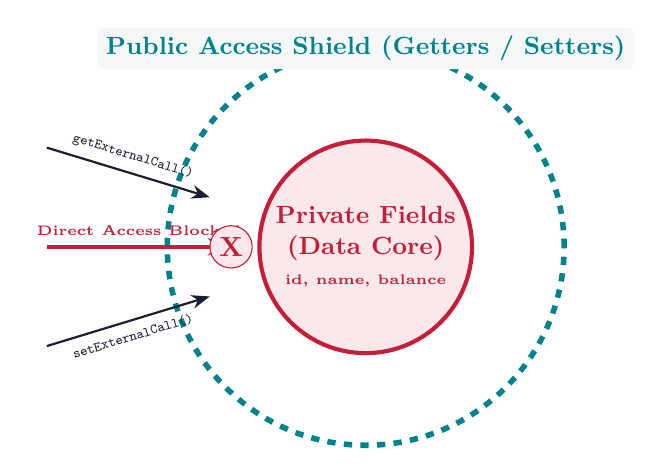
\begin{tikzpicture}[scale=0.9]
  % Inner Core (Private Data)
  \draw[draw=myred, fill=hdrred, line width=1.5pt] (0,0) circle (1.5);
  \node[align=center, color=myred, font=\small\bfseries] at (0,0) {Private Fields\\(Data Core)\\{\tiny id, name, balance}};

  % Outer Ring (Public Access methods)
  \draw[draw=myteal, fill=none, line width=2pt, dashed] (0,0) circle (2.8);
  \node[color=myteal, font=\small\bfseries, fill=mygray, inner sep=3pt, rounded corners=2pt] at (0, 2.8) {Public Access Shield (Getters / Setters)};

  % Arrows representing external calls
  \draw[arrow] (-4.5, 1.4) -- (-2.2, 0.7) node[midway, sloped, above, font=\tiny] {\texttt{getExternalCall()}};
  \draw[arrow] (-4.5, -1.4) -- (-2.2, -0.7) node[midway, sloped, below, font=\tiny] {\texttt{setExternalCall()}};
  
  % Blocked direct access
  \draw[redarrow, line width=1.2pt] (-4.5, 0) -- (-1.9, 0) node[midway, above, font=\tiny\bfseries] {Direct Access Blocked};
  \node[draw=myred, fill=hdrred, circle, inner sep=1.5pt] at (-1.9,0) {\color{myred}\textbf{X}};
\end{tikzpicture}
\tcbset{after={\color{black}}}
\end{tcolorbox}

% ===============================================================================
\section{Inheritance and Reuse Models}
% ===============================================================================

Inheritance enables hierarchical classifications. In Java, classes are extended using the \texttt{extends} keyword.

\begin{tcolorbox}[defbox, title={\textbf{Inheritance Characteristics}}]
\begin{itemize}[leftmargin=*, itemsep=3pt]
  \item \textbf{Single Inheritance Only:} Java classes can only extend \textbf{one} parent class to prevent the diamond problem (ambiguity under duplicate variable/method signatures).
  \item \textbf{The \texttt{super} Keyword:} Used to invoke the parent class constructor (must be the first statement in the subclass constructor), access overridden parent methods, or read hidden parent variables.
\end{itemize}
\end{tcolorbox}

\begin{tcolorbox}[tikzbox, title={Inheritance Trees supported in Java}]
\centering
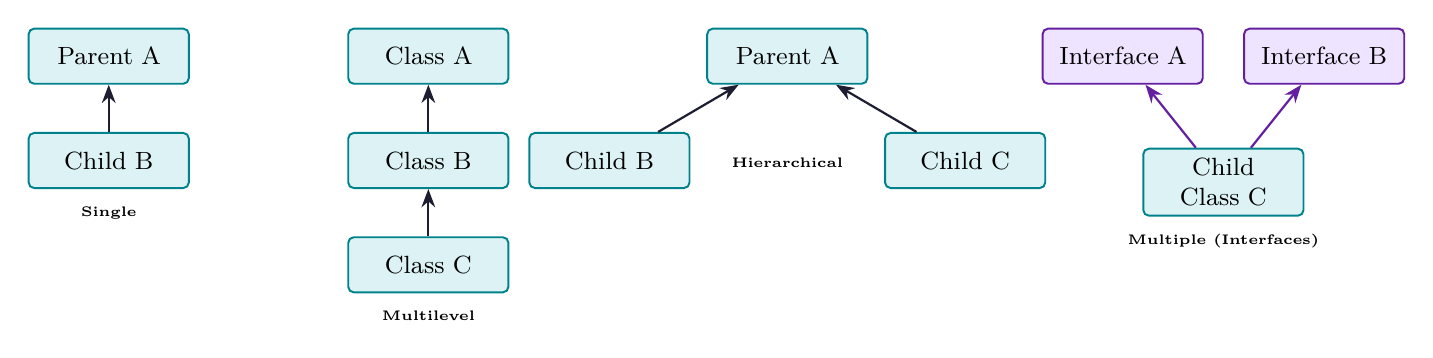
\begin{tikzpicture}[node distance=1.0cm and 1.8cm,
  cls/.style={rectangle, draw=myteal, fill=hdrteal, text width=1.8cm,
    align=center, minimum height=0.7cm, font=\small, rounded corners=2pt, line width=0.7pt},
  intf/.style={rectangle, draw=mypurple, fill=hdrpurple, text width=1.8cm,
    align=center, minimum height=0.7cm, font=\small, rounded corners=2pt, line width=0.7pt}]

  % --- Single ---
  \node[cls] (S1) {Parent A};
  \node[cls, below=0.6cm of S1] (S2) {Child B};
  \draw[arrow] (S2) -- (S1);
  \node[below=0.1cm of S2, font=\tiny\bfseries] {Single};

  % --- Multilevel ---
  \node[cls, right=2.0cm of S1] (M1) {Class A};
  \node[cls, below=0.6cm of M1] (M2) {Class B};
  \node[cls, below=0.6cm of M2] (M3) {Class C};
  \draw[arrow] (M3) -- (M2);
  \draw[arrow] (M2) -- (M1);
  \node[below=0.1cm of M3, font=\tiny\bfseries] {Multilevel};

  % --- Hierarchical ---
  \node[cls, right=2.5cm of M1] (H1) {Parent A};
  \node[cls, below left=0.6cm and 0.2cm of H1] (H2) {Child B};
  \node[cls, below right=0.6cm and 0.2cm of H1] (H3) {Child C};
  \draw[arrow] (H2) -- (H1);
  \draw[arrow] (H3) -- (H1);
  \node[below=0.8cm of H1, font=\tiny\bfseries] {Hierarchical};

  % --- Multiple (via Interfaces) ---
  \node[intf, right=2.2cm of H1] (I1) {Interface A};
  \node[intf, right=0.5cm of I1] (I2) {Interface B};
  \node[cls, below=0.8cm of $(I1.south)!0.5!(I2.south)$] (I3) {Child Class C};
  \draw[arrow, color=mypurple] (I3) -- (I1);
  \draw[arrow, color=mypurple] (I3) -- (I2);
  \node[below=0.1cm of I3, font=\tiny\bfseries] {Multiple (Interfaces)};
\end{tikzpicture}
\end{tcolorbox}

\subsection{Composition vs. Inheritance}
Design patterns advocate favoring object composition over class inheritance:

\par\noindent
{\renewcommand{\arraystretch}{1.5}%
\begin{tabularx}{\linewidth}{|B{3.2cm}|Y|Y|}
\hline
\textbf{Metric} & \textbf{Composition (Has-A Relationship)} & \textbf{Inheritance (Is-A Relationship)} \\
\hline
\textbf{Coupling Level} & Loose coupling; internal details remain private. & Tight coupling; breaks encapsulation boundary. \\
\hline
\textbf{Flexibility} & Behaviors can change dynamically at runtime. & Static; behavior fixed at compilation time. \\
\hline
\textbf{Design Reuse} & Reuses functional components as class members. & Reuses code by expanding a class hierarchy. \\
\hline
\textbf{Example} & \texttt{Car} has an \texttt{Engine} instance. & \texttt{Car} is a subclass of \texttt{Vehicle}. \\
\hline
\end{tabularx}}

% ===============================================================================
\section{Polymorphism and Runtime Resolution}
% ===============================================================================

\subsection{Method Overloading vs. Overriding}
These represent static and dynamic polymorphism:

\par\noindent
{\renewcommand{\arraystretch}{1.5}%
\begin{tabularx}{\linewidth}{|B{3.0cm}|Y|Y|}
\hline
\textbf{Feature} & \textbf{Method Overloading (Static)} & \textbf{Method Overriding (Dynamic)} \\
\hline
\textbf{Class Context} & Occurs within the same class definition. & Occurs across child-parent subclass hierarchy. \\
\hline
\textbf{Method Signature} & Name must be same; parameters must differ. & Signature (parameters, returns) must match. \\
\hline
\textbf{Resolution Time} & Compile-time (static binding). & Runtime (dynamic binding). \\
\hline
\textbf{Keywords} & None required. & Assisted by \texttt{@Override} annotation. \\
\hline
\end{tabularx}}

\subsection{Dynamic Method Dispatch}
Dynamic Method Dispatch is the mechanism by which a call to an overridden method is resolved at runtime rather than compile-time.

\begin{tcolorbox}[defbox, title={\textbf{Dynamic Method Dispatch Rule}}]
When an overridden method is called through a superclass reference, Java determines which version of the method to execute based on the \textbf{type of the actual object} being referred to at runtime, not the type of the reference variable.
\end{tcolorbox}

\begin{tcolorbox}[tikzbox, title={Dynamic Method Dispatch Flow}]
\centering
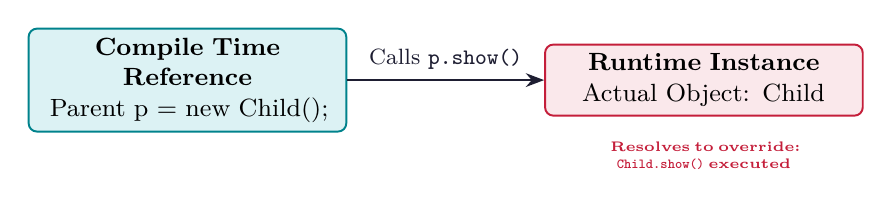
\begin{tikzpicture}[node distance=1.5cm and 2.5cm,
  refnode/.style={rectangle, draw=myteal, fill=hdrteal, text width=3.8cm,
    align=center, minimum height=0.8cm, font=\small, rounded corners=3pt, line width=0.7pt},
  instnode/.style={rectangle, draw=myred, fill=hdrred, text width=3.8cm,
    align=center, minimum height=0.8cm, font=\small, rounded corners=3pt, line width=0.7pt}]

  % Compilation (Reference Type)
  \node[refnode] (ref) {\textbf{Compile Time Reference}\\{\small Parent p = new Child();}};
  
  % Runtime Target (Instance Type)
  \node[instnode, right=of ref] (inst) {\textbf{Runtime Instance}\\{\small Actual Object: Child}};

  % Method call
  \draw[arrow] (ref) -- (inst) node[midway, above, font=\footnotesize] {Calls \texttt{p.show()}};
  
  % Resolution
  \node[below=0.2cm of inst, font=\tiny\bfseries, color=myred, align=center, text width=3.8cm] {Resolves to override:\\\texttt{Child.show()} executed};
\end{tikzpicture}
\end{tcolorbox}

% ===============================================================================
\section{Interfaces, Abstract Classes, and Access Modifiers}
% ===============================================================================

\subsection{Abstract Class vs. Interface}
These constructs provide different levels of abstraction:

\par\noindent
{\renewcommand{\arraystretch}{1.5}%
\begin{tabularx}{\linewidth}{|B{3.2cm}|Y|Y|}
\hline
\textbf{Feature} & \textbf{Abstract Class} & \textbf{Interface} \\
\hline
\textbf{Multiple Inheritance} & Allowed to inherit only one abstract parent. & A class can implement multiple interfaces. \\
\hline
\textbf{State Variables} & Can contain instance variables (stateful). & Variables must be \texttt{public static final}. \\
\hline
\textbf{Methods} & Concrete methods and abstract methods. & Abstract methods (pre-Java 8), defaults allowed. \\
\hline
\textbf{Keywords} & Declared with \texttt{abstract class} and \texttt{extends}. & Declared with \texttt{interface} and \texttt{implements}. \\
\hline
\end{tabularx}}

\subsection{Access Modifiers}
Java regulates visibility using four access levels:
\begin{itemize}[leftmargin=*, itemsep=3pt]
  \item \textbf{\texttt{private}:} Visible only within the declaring class.
  \item \textbf{Default (no modifier):} Visible only to classes inside the same package.
  \item \textbf{\texttt{protected}:} Visible to the same package and subclass child files in external packages.
  \item \textbf{\texttt{public}:} Accessible from any class anywhere in the project.
\end{itemize}

% ===============================================================================
\section{Object Class and SOLID Design Principles}
% ===============================================================================

\subsection{The Root Object Class}
Every Java class implicitly extends \texttt{java.lang.Object}. It defines essential methods:
\begin{itemize}[leftmargin=*, itemsep=3pt]
  \item \textbf{\texttt{toString()}:} Returns a string representation of the object (ClassName@HexHashCode).
  \item \textbf{\texttt{equals(Object obj)}:} Compares reference equality. Overridden to compare values.
  \item \textbf{\texttt{hashCode()}:} Returns an integer hash code mapped to the object's memory address.
  \item \textbf{\texttt{clone()}:} Creates a field-by-field copy of the current object.
\end{itemize}

\subsection{SOLID Design Principles}
These principles ensure Java classes are maintainable:
\begin{itemize}[leftmargin=*, itemsep=4pt]
  \item \textbf{Single Responsibility Principle (SRP):} A class must have exactly one reason to change.
  \item \textbf{Open/Closed Principle (OCP):} Software entities should be open for extension, closed for modification.
  \item \textbf{Liskov Substitution Principle (LSP):} Derived classes must be fully substitutable for their base classes.
  \item \textbf{Interface Segregation Principle (ISP):} Clients should not be forced to depend on interfaces they do not use.
  \item \textbf{Dependency Inversion Principle (DIP):} Depend on abstractions, not concrete implementations.
\end{itemize}

\newpage
% ===============================================================================
\begin{center}
  {\large\bfseries\color{myred} Quick Revision --- Module 3}\\[3pt]
  {\small\color{mydark} OOP Principles, Inheritance, Polymorphism, Packages \& Interfaces $|$ OE-EC704A}
\end{center}
\noindent{\color{myred}\rule{\linewidth}{1.2pt}}
\vspace{4pt}

\begin{tcolorbox}[formulabox, title={\textbf{Inheritance, Packages \& Interface Syntax}}]
{\renewcommand{\arraystretch}{1.3}%
\begin{tabularx}{\linewidth}{l Y}
\textbf{Concept} & \textbf{Syntax and Structural Format} \\
\hline
Subclass Extension & \texttt{class Child extends Parent \{ ... \}} \\
Super Constructor Call & \texttt{Child(int val) \{ super(val); ... \}} \\
Interface Declaration & \texttt{interface Flyable \{ void fly(); \}} \\
Interface Implementation & \texttt{class Bird implements Flyable \{ public void fly() \{ ... \} \}} \\
\hline
\textbf{Package Syntax} & \textbf{Access and Import Declarations} \\
\hline
Package Header & \texttt{package com.cgec.webtech;} \\
Import Header & \texttt{import com.cgec.webtech.MyClass;} \\
Abstract Method & \texttt{abstract void calculateScore();} \\
Constant in Interface & \texttt{int MAX\_RETRY = 5; // Public static final by default} \\
\end{tabularx}}
\end{tcolorbox}

\begin{tcolorbox}[defbox, title={\textbf{One-Line Definitions}}]
\begin{itemize}[leftmargin=*, itemsep=2pt]
  \item \textbf{Inheritance:} The mechanism by which a subclass inherits variables and methods from a superclass.
  \item \textbf{Method Overloading:} Declaring methods with the same name but different parameters in one class.
  \item \textbf{Method Overriding:} Declaring a method in a subclass with the same signature as in the parent class.
  \item \textbf{Dynamic Method Dispatch:} Dynamic binding resolution that determines overridden method calls at runtime.
  \item \textbf{Abstract Class:} A class that cannot be instantiated and may contain abstract methods.
  \item \textbf{Interface:} A contract defining empty method signatures that implementing classes must satisfy.
  \item \textbf{Package:} A namespace group containing related classes, interfaces, and packages.
  \item \textbf{SOLID:} A set of five object-oriented design principles for readable and maintainable software.
\end{itemize}
\tcbset{after={\color{black}}}
\end{tcolorbox}

\begin{tcolorbox}[exambox, title={\textbf{Frequently Asked / Viva Questions}}]
\begin{enumerate}[leftmargin=*, label=\textbf{Q\arabic*.}, itemsep=5pt]
  \item \Q{Why does Java not support multiple inheritance with classes?}
        To avoid the diamond problem. If class C extends both class A and class B, and both parents define a method with the same signature \texttt{show()}, class C cannot determine which parent version to inherit.
        
  \item \Q{How does Java support multiple inheritance then?}
        Java allows a class to implement multiple interfaces. Since interfaces do not hold instance state and their methods were traditionally empty, there is no duplicate implementation ambiguity.
        
  \item \Q{What is the difference between \texttt{this()} and \texttt{super()} constructor calls?}
        \texttt{this()} invokes another constructor within the same class. \texttt{super()} invokes a constructor of the parent superclass. Both must be the first line of their respective constructors.
        
  \item \Q{Can an abstract class have constructors? Why?}
        Yes. Although an abstract class cannot be instantiated directly, its constructor is called during subclass instantiation via \texttt{super()} to initialize its fields.
        
  \item \Q{What is the difference between \texttt{final} class, \texttt{final} method, and \texttt{final} variable?}
        A \texttt{final} class cannot be inherited. A \texttt{final} method cannot be overridden. A \texttt{final} variable behaves as a constant and cannot be reassigned.
        
  \item \Q{What is the contract between \texttt{equals()} and \texttt{hashCode()}?}
        If two objects are equal according to \texttt{equals()}, they must return the same integer hash code from \texttt{hashCode()}. If overridden, both must be updated to preserve this rule.
        
  \item \Q{What is the difference between composition and inheritance?}
        Inheritance represents an IS-A relationship and creates tight coupling. Composition represents a HAS-A relationship, wrapping objects to provide loose coupling.
        
  \item \Q{How does the access level of a subclass method override compare to the parent class method?}
        An overriding method cannot restrict the access level of the overridden parent method. For example, a \texttt{protected} method in a parent class can only be overridden as \texttt{protected} or \texttt{public}.
        
  \item \Q{What are default methods in interfaces and why were they introduced in Java 8?}
        Default methods have an implementation inside the interface using the \texttt{default} keyword. They allow adding new methods to interfaces without breaking existing implementing classes.
        
  \item \Q{What is the difference between compile-time and runtime polymorphism?}
        Compile-time polymorphism (overloading) resolves method calls during compilation using static binding. Runtime polymorphism (overriding) resolves method calls during execution using dynamic binding.
\end{enumerate}
\end{tcolorbox}

\begin{tcolorbox}[tikzbox, title={Java Access Modifier Visibility Matrix}]
\centering
{\renewcommand{\arraystretch}{1.45}%
\begin{tabularx}{\linewidth}{|B{2.8cm}|>{\centering\arraybackslash}X|>{\centering\arraybackslash}X|>{\centering\arraybackslash}X|>{\centering\arraybackslash}X|}
\hline
\textbf{Modifier} & \textbf{Same Class} & \textbf{Same Package} & \textbf{Subclass} & \textbf{Everywhere} \\
\hline
\textbf{\texttt{private}} & Yes & No & No & No \\
\hline
\textbf{Default} & Yes & Yes & No & No \\
\hline
\textbf{\texttt{protected}} & Yes & Yes & Yes & No \\
\hline
\textbf{\texttt{public}} & Yes & Yes & Yes & Yes \\
\hline
\end{tabularx}}
\end{tcolorbox}

\end{document}
